% This work is licensed under the Creative Commons Attribution-NonCommercial 4.0 International License.
% To view a copy of this license, visit http://creativecommons.org/licenses/by-nc/4.0/
% or send a letter to Creative Commons, PO Box 1866, Mountain View, CA 94042, USA.

% !TEX TS-program = xelatex

\documentclass[../Main/chem371-notes.tex]{subfiles}

\setcounter{chapter}{2}
\begin{document}

\chapter{Hartree--Fock Theory}

\section{Hartree--Fock theory and the independent particle approximation}
The simplest quantum chemistry method is the Hartree--Fock approach.
This method relies on an independent particle approximation, where the wave function is expressed as a product of wave functions of single electron (orbitals).
We will indicate orbitals with the lower-case Greek letter phi ($\varphi$).
An orbital is a function of the coordinate vector $\mathbf{r} = (x,y,z)$ for an electron.
To distinguish between different orbitals we will label them with an index and write them as
\begin{iequation}
\varphi_i(\mathbf{r})
\end{iequation}

In the Hartree--Fock approach we approximate the wave function of $N$ electrons as a product of the orbitals for each electron
\begin{equation}
\label{eq:hartree_prod}
\Psi(\mathbf{r}_1, \mathbf{r}_2, \ldots, \mathbf{r}_N) \approx \varphi_1(\mathbf{r}_1) \varphi_2(\mathbf{r}_2) \cdots \varphi_N(\mathbf{r}_N)
\end{equation}
This approximation is convenient because it breaks down the problem of solving the Schr\"{o}dinger for a wave function of $3N$ coordinates into a simpler problem where we solve $N$ times for wave functions of 3 coordinates.\mnote{For example, imagine that you represent the wave function $\Psi(\mathbf{r}_1, \mathbf{r}_2, \ldots, \mathbf{r}_N)$ using a grid that has 10 points along each dimension.
For $N$ electrons, this grid will have a total of $10^{3N}$ points since $\Psi$ depends on $3N$ coordinates.
In comparison, if we represent each orbital with the same grid, each orbital requires only $10^3$ grid points, and the total number of grid points is $N 10^3$.
Even for as little as six electrons the exact wave function required already $10^{18}$ points, while the Hartree--Fock approach requires only $6000$!
} 
This simplification makes Hartree--Fock theory much more affordable than a direct solution of the Schr\"{o}dinger equation!

\section{Spin and the Pauli principle (antisymmetry)}
The wave function form of Eq.~\eqref{eq:hartree_prod} is still missing two important ingredients: it does not account for the spin of electrons and the Pauli exclusion principle.

Spin can be easily introduced by recognizing that each orbital must be accompanied by a spin function, that is, a label for the spin of the electron.
As you have learned from previous classes, the electron can have to value of spin: up (alpha, $\alpha$) and down (beta, $\beta$).
%\mnote{
%\begin{equation}
%\varphi_i(\mathbf{r}) \alpha \equiv 
%\begin{tikzpicture}[
%	baseline={([yshift=-.5ex]current bounding box.center)},
%	vertex/.style={anchor=base, minimum size=18pt, inner sep=2pt}]
%%    \draw (0.25,0.5) circle (0.4);
%    \draw (0,0.5) -- (0.5,0.5);
%    \draw[thick,->,>=stealth] (0.15,0.325) -- (0.15,0.675);
%%    \draw[thick,<-,>=stealth] (0.35,0.325) -- (0.35,0.675);    
%  \end{tikzpicture}
%\end{equation}
%}
So if we want to specify that an electron occupies orbital $\varphi_i$ and has spin alpha we write $\varphi_i(\mathbf{r}) \alpha$, which is equivalent to the in the arrow notation to
\begin{equation}
\varphi_i(\mathbf{r}) \alpha
\equiv \;
\begin{tikzpicture}[baseline={([yshift=-.5ex]current bounding box.center)},]
    \draw (0,0.5) -- (0.5,0.5);
    \draw[thick,->,>=stealth] (0.15,0.325) -- (0.15,0.675);
\end{tikzpicture}
\end{equation}
For an electron with beta spin we similarly write
\begin{equation}
\varphi_i(\mathbf{r}) \beta
\equiv \;
\begin{tikzpicture}[baseline={([yshift=-.5ex]current bounding box.center)},]
    \draw (0,0.5) -- (0.5,0.5);
    \draw[thick,<-,>=stealth] (0.35,0.325) -- (0.35,0.675);    
\end{tikzpicture}
\end{equation}
When we don not want to be specific about the spin of the electron (and thus allow for both options), we will use instead the \emph{spinorbital} notation based on the Greek letter psi [$\psi(x)$] and use the variable $x = \{ \mathbf{r},\sigma\}$ to represent both the position vector ($\mathbf{r}$) and one spin coordinate ($\omega$).
For the moment, we can think of spin orbitals as always coming in alpha/beta pairs that share the same spatial orbital
\begin{align}
\psi_i(x) & = \varphi_i(\mathbf{r}) \alpha \\
\psi_{\bar{i}}(x) & = \varphi_i(\mathbf{r}) \beta
\end{align}
Now we can be more precise and write the product wave function as
\begin{equation}
\label{eq:hartree_prod_spin}
\Psi(x_1, x_2, \ldots, x_N) \approx \psi_1(x_1) \psi_{\bar{1}}(x_2) \cdots
\end{equation}

Equation~\eqref{eq:hartree_prod_spin} is still not fully correct.
To make sure that the wave function satisfies the Pauli exclusion principle, we have to enforce that the sign of $\Psi(x_1, x_2, \ldots, x_N)$ changes if we exchange the labels of any two particles.
To illustrate this point, consider two electrons. The wave function $\Psi(x_1, x_2)$ depends on the position and spin of each electron ($x_1$, $x_2$), and it must change sign when we replace $x_2$ with $x_1$ and vice versa, which means
\begin{iequation}
\Psi(x_1, x_2) = -\Psi(x_2, x_1)
\end{iequation}
It is easy to write down a wave function built from orbitals that satisfies this condition, it just requires making the product antisymmetric with respect to the coordinates.
Such a wave function is called a \emph{Slater determinant}\mnote{
The Slater determinant is named for John C. Slater, who introduced the determinant in 1929 as a means of ensuring the antisymmetry of a many-electron wave function, although the wave function in the determinant form first appeared independently in Heisenberg's and Dirac's articles three years earlier.  (Source: Wikipedia)
\begin{center}
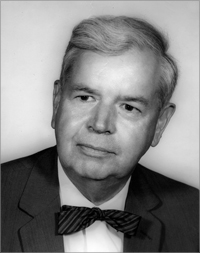
\includegraphics[width=1.5in]{img/slater_john_clarke_a3.jpg}
\end{center}
\captionof{figure}{John C. Slater.}
} and for the two electron case is it written as\mnote{Here I use the symbol $\ket{\psi_i \psi_j \cdots }$ to indicate a general Slater determinant.}
\begin{iequation}
\Psi_{\mathrm{SD}}(x_1,x_2) =
\ket{\psi_i \psi_j}
%\frac{1}{\sqrt{2}} 
%\begin{vmatrix}
%\psi_1(x_1) & \psi_1(x_2) \\
%\psi_2(x_1) & \psi_2(x_2)
%\end{vmatrix}
= \frac{1}{\sqrt{2}} \left[ \psi_i(x_1)\psi_j(x_2) - \psi_i(x_2)\psi_j(x_1) \right]
\end{iequation}
Stater determinants correspond exactly to the orbital diagrams with orbitals filled with electrons (represented by arrows).
For example, the electron configuration with two electrons filling the same orbital corresponds to the following Slater determinant\begin{equation}
\ket{\psi_1 \psi_{\bar{1}}} = 
\ket{\varphi_1 \alpha \varphi_1 \beta }
\equiv \;
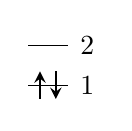
\begin{tikzpicture}[baseline={([yshift=-.5ex]current bounding box.center)},]
    \draw (0,0.5) -- (0.5,0.5);
    \draw[thick,->,>=stealth] (0.15,0.325) -- (0.15,0.675);    
    \draw[thick,<-,>=stealth] (0.35,0.325) -- (0.35,0.675);    
    \draw (0,1.0) -- (0.5,1.0);
    \draw (0.75,0.5) node{1};
    \draw (0.75,1.0) node{2};
\end{tikzpicture}
\end{equation}
This electron arrangement is called a \emph{closed shell}, because all the electrons are paired. It corresponds to a \emph{singlet} electronic state.

However, we could also arrange the electrons in two different orbitals both with alpha spin in an \emph{open-shell} configuration
\begin{equation}
\ket{\psi_1 \psi_2}= 
\ket{\varphi_1 \alpha \varphi_2\alpha}
\equiv \;
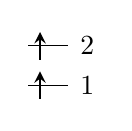
\begin{tikzpicture}[baseline={([yshift=-.5ex]current bounding box.center)},]
    \draw (0,0.5) -- (0.5,0.5);
    \draw[thick,->,>=stealth] (0.15,0.325) -- (0.15,0.675);    
    \draw[thick,->,>=stealth] (0.15,0.825) -- (0.15,1.175);        
    \draw (0,1.0) -- (0.5,1.0);
    \draw (0.75,0.5) node{1};
    \draw (0.75,1.0) node{2};
\end{tikzpicture}
\end{equation}
In this state, the spin of the electrons add up and we get what is called a \emph{triplet state}.

We have covered a lot of details in this section, so I want to make sure that the important message comes across: \emph{in the Hartree--Fock method the wave function of many electrons is approximated with a single Slater determinant}.
This approach satisfies the Pauli exclusion principle and it has a direct connection to the familiar orbital diagrams.

\section{The Hartree--Fock equation}
The main goal of the Hartree--Fock method is to find the orbitals that give the ``best'' possible wave function.
Here by ``best'' we mean precisely the one that minimizes the expectation value of the energy, which is given by the integral
\begin{equation}
E_\mathrm{SD} = \int \Psi_{\mathrm{SD}}^* \hat{H}\Psi_{\mathrm{SD}}
\end{equation}
The \emph{variational} theorem guarantees that the energy of an approximate wave function $\tilde{\Psi}$ is always greater than the exact energy, $\tilde{E} \geq E_\mathrm{exact}$, and the closer we get to the exact energy $E_\mathrm{exact}$, the better our wave function $\tilde{\Psi}$ approximate the exact solution $\Psi_\mathrm{exact}$.

The orbitals that minimize the energy satisfy the \emph{Hartree--Fock equations}
\begin{equation}
\hat{f} \psi_i(x) = \epsilon_i  \psi_i(x), \quad \text{ for all } \psi_i(x)
\end{equation}
where $\hat{f}$ is the \emph{Fock operator}.
This is an eigenvalue equation like the Schr\"{o}dinger equation, but it is simpler because it only involves one orbital at the time (a functions of 3 coordinates only).
However, it is important to remember that this equation is valid only in the Hartree--Fock approximation.
The quantity $\epsilon_i$ is called the \emph{orbital energy} and it is the eigenvalue corresponding to the orbital $\psi_i$.

The physical interpretation of the Hartree--Fock equation is that we can approximate the interaction (repulsion) of an electron in orbital $\psi_i$ with all the remaining $N-1$ electrons via an average potential. This potential is included in the Fock operator
\begin{equation}
\hat{f} = \underbrace{-\frac{1}{2}\nabla^2}_{\text{kinetic}}
+\underbrace{
- \sum_i^{\mathrm{nuclei}} \frac{Z_i}{|\mathbf{r} - \mathbf{R}_i|}
}_{\text{electron-nuclear}}
+
\underbrace{
\int d\mathbf{r}' \, \frac{\rho(\mathbf{r}')}{|\mathbf{r} -\mathbf{r}'|}
}_{\text{Coulomb interaction}} + \text{ exchange interaction}
\end{equation}
in the terms that depend on the density of electrons ($\rho$).
The electron density is in turn given by the sum of the square of the occupied orbitals, which for a closed-shell molecule is given by
\begin{equation}
\rho(\mathbf{r}) = 2 \sum_{i}^\mathrm{occupied} |\varphi(\mathbf{r})|^2
\end{equation}
The Hartree--Fock equations and these last two equations tell us that to find the orbital we need to know $\hat{f}$, but to know $\hat{f}$ we need to know the density, which is determined by the orbitals.
In practice this means that the Hartree--Fock equations have to be solved via an iterative \emph{self-consistent-field (SCF) procedure}.

This procedure consists of the following steps:
\begin{enumerate}
\item Forming an initial guess. At beginning of an SCF procedure we need to start from orbitals that are close to the optimal ones.
Common ways to guess the orbitals include neglecting electron repulsion or forming the average potential from a superposition of atomic densities.
\item Updating the Fock matrix. Using the current set of orbitals, the average potential and the Fock operator are built. 
\item Determining the orbitals and orbital energies. Using the current Fock matrix, the Hartree--Fock equations are solved to obtain one set of orbitals and orbital energies and an updated value for the total energy.
\item Convergence check. The program checks if the change in energy and orbitals with respect to the previous iteration is less than a predefined convergence threshold. If the computation has converged, we stop. Otherwise, we go back to step 2. and use the new set of orbital to compute a new Fock operator.
\end{enumerate}

The following is the output of a Hartree--Fock computation on water.
In this example, the iterations start with a guess of the density given by the superposition of atomic densities (SAD)\mnote{Computational chemists love acronyms. With time you will become conversant with this language.}
As the iterations progress, the energy becomes lower and lower (in accordance with the variational principle) and we reach convergence in eight iterations to the final value $-76.02665366185$ \Eh.
Note that in the last step the energy is converged to $-5.4 \times 10^{-10}$ \Eh.\mnote{Quantum chemistry computations are usually converged to high accuracy. It is not uncommon to see the energy optimized to less than $10^{-7}$--$10^{-8}$ \Eh, and in certain cases down to even $10^{-12}$ \Eh.

The quantity labeled ``RMS |[F,P]|'' measures the derivative of the energy, and it is another way to monitor the convergence (remember that at a minimum, the gradient is zero).
The label ``DIIS'', indicates that the code is using the direct inversion of the iterative subspace (DIIS) algorithm to accelerate the convergence.}
\begin{small}
\begin{verbatim}
  Water/Hartree-Fock
  ==> Iterations <==
                   Total Energy       Delta E     RMS |[F,P]|

@RHF iter SAD:   -75.50773245935   -7.55077e+01   0.00000e+00 
@RHF iter   1:   -75.95378451304   -4.46052e-01   3.03072e-02 DIIS
@RHF iter   2:   -76.00708060915   -5.32961e-02   1.73589e-02 DIIS
@RHF iter   3:   -76.02624491762   -1.91643e-02   1.58426e-03 DIIS
@RHF iter   4:   -76.02663310976   -3.88192e-04   3.65265e-04 DIIS
@RHF iter   5:   -76.02665270339   -1.95936e-05   6.70876e-05 DIIS
@RHF iter   6:   -76.02665363515   -9.31757e-07   1.06688e-05 DIIS
@RHF iter   7:   -76.02665366131   -2.61654e-08   1.50538e-06 DIIS
@RHF iter   8:   -76.02665366185   -5.39330e-10   3.50179e-07 DIIS
  Energy and wave function converged.
\end{verbatim}
\end{small}


\section{Interpretation of the orbital energies}

It is important to understand the precise meaning of the orbital energies $\epsilon_i$ because it is slightly different than our intuition as chemists.
\emph{Koopmans' theorem} shows that the orbital energies are related to the energy necessary to remove or add electrons to an orbital.
More precisely, for orbitals that are occupied by electrons, Koopmans' theorem says that $-\epsilon_i$ correspond to the energy necessary to remove one electron (ionize) from the system
\begin{center}
\ce{M -> M+ + e-}
\end{center}
Koopmans' theorem can be stated as
\begin{iequation}
\text{Ionization potential for electron in }\psi_i = \mathrm{IP}_i = E^{N-1} - E^{N} = -\epsilon_i.
\end{iequation}
If an occupied orbital has a negative energy, then we have to put energy into a molecule to remove that electron (the IP is positive).

\mfigure{
\begin{center}
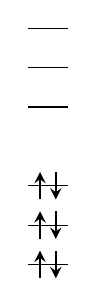
\begin{tikzpicture}[baseline={([yshift=-.5ex]current bounding box.center)},]
    \draw (0,0.5) -- (0.5,0.5);
    \draw[thick,->,>=stealth] (0.15,0.325) -- (0.15,0.675);    
    \draw[thick,<-,>=stealth] (0.35,0.325) -- (0.35,0.675);    
    \draw (0,1.0) -- (0.5,1.0);
    \draw[thick,->,>=stealth] (0.15,0.825) -- (0.15,1.175);    
    \draw[thick,<-,>=stealth] (0.35,0.825) -- (0.35,1.175);    
    \draw (0,1.5) -- (0.5,1.5);
    \draw[thick,->,>=stealth] (0.15,1.325) -- (0.15,1.675);    
    \draw[thick,<-,>=stealth] (0.35,1.325) -- (0.35,1.675);   
    \draw (0,2.5) -- (0.5,2.5);
    \draw (0,3.0) -- (0.5,3.0);
    \draw (0,3.5) -- (0.5,3.5);
%    \draw (0.75,0.5) node{1};
%    \draw (0.75,1.0) node{2};
\end{tikzpicture}
\ce{->}
\begin{tikzpicture}[baseline={([yshift=-.5ex]current bounding box.center)},]
    \draw (0,0.5) -- (0.5,0.5);
    \draw[thick,->,>=stealth] (0.15,0.325) -- (0.15,0.675);    
    \draw[thick,<-,>=stealth] (0.35,0.325) -- (0.35,0.675);    
    \draw (0,1.0) -- (0.5,1.0);
    \draw[thick,->,>=stealth] (0.15,0.825) -- (0.15,1.175);    
    \draw[thick,<-,>=stealth] (0.35,0.825) -- (0.35,1.175);    
    \draw (0,1.5) -- (0.5,1.5);
%    \draw[thick,->,>=stealth] (0.15,1.325) -- (0.15,1.675);    
    \draw[thick,<-,>=stealth] (0.35,1.325) -- (0.35,1.675);   
    \draw (0,2.5) -- (0.5,2.5);
    \draw (0,3.0) -- (0.5,3.0);
    \draw (0,3.5) -- (0.5,3.5);
    \draw (1.25,1.5) node{IP = $-\epsilon_i$};
%    \draw (0.75,1.0) node{2};
\end{tikzpicture}
\\ \vspace{24pt}
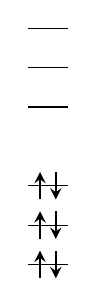
\begin{tikzpicture}[baseline={([yshift=-.5ex]current bounding box.center)},]
    \draw (0,0.5) -- (0.5,0.5);
    \draw[thick,->,>=stealth] (0.15,0.325) -- (0.15,0.675);    
    \draw[thick,<-,>=stealth] (0.35,0.325) -- (0.35,0.675);    
    \draw (0,1.0) -- (0.5,1.0);
    \draw[thick,->,>=stealth] (0.15,0.825) -- (0.15,1.175);    
    \draw[thick,<-,>=stealth] (0.35,0.825) -- (0.35,1.175);    
    \draw (0,1.5) -- (0.5,1.5);
    \draw[thick,->,>=stealth] (0.15,1.325) -- (0.15,1.675);    
    \draw[thick,<-,>=stealth] (0.35,1.325) -- (0.35,1.675);   
    \draw (0,2.5) -- (0.5,2.5);
    \draw (0,3.0) -- (0.5,3.0);
    \draw (0,3.5) -- (0.5,3.5);
%    \draw (0.75,0.5) node{1};
%    \draw (0.75,1.0) node{2};
\end{tikzpicture}
\ce{->}
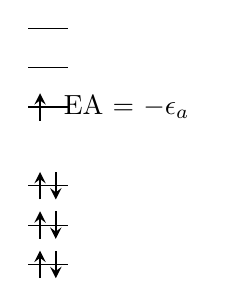
\begin{tikzpicture}[baseline={([yshift=-.5ex]current bounding box.center)},]
    \draw (0,0.5) -- (0.5,0.5);
    \draw[thick,->,>=stealth] (0.15,0.325) -- (0.15,0.675);    
    \draw[thick,<-,>=stealth] (0.35,0.325) -- (0.35,0.675);    
    \draw (0,1.0) -- (0.5,1.0);
    \draw[thick,->,>=stealth] (0.15,0.825) -- (0.15,1.175);    
    \draw[thick,<-,>=stealth] (0.35,0.825) -- (0.35,1.175);    
    \draw (0,1.5) -- (0.5,1.5);
    \draw[thick,->,>=stealth] (0.15,1.325) -- (0.15,1.675);    
    \draw[thick,<-,>=stealth] (0.35,1.325) -- (0.35,1.675);   
    \draw (0,2.5) -- (0.5,2.5);
    \draw[thick,->,>=stealth] (0.15,2.325) -- (0.15,2.675);        
    \draw (0,3.0) -- (0.5,3.0);
    \draw (0,3.5) -- (0.5,3.5);
    \draw (1.25,2.5) node{EA = $-\epsilon_a$};
%    \draw (0.75,1.0) node{2};
\end{tikzpicture}
\end{center}
\captionof{figure}{Illustration of Koopmans' theorem.}
\label{fig:koopmans}
}

Similarly, for orbitals that are not occupied, the orbital energy $\epsilon_a$ corresponds to the energy released when an electron is added to form an anion (if the starting molecule is neutral)
\begin{center}
\ce{M + e- -> M-}
\end{center}
In this case, Koopmans' theorem helps us quantify the electron affinity
\begin{iequation}
\text{Electron affinity for electron in }\psi_a = \mathrm{EA}_a = E^{N} - E^{N+1} = -\epsilon_a.
\end{iequation}
Therefore, if an unoccupied orbital has a negative energy (positive EA), a molecule will attach an electron and form a stable negative ion.
If instead $\epsilon_a$ is positive, a molecule will not accept an electron, and its anion will be unstable with respect to self ionization (the anion will spontaneously loose an electron in a finite amount of time).

Koopmans' theorem assumes that during the electron ionization/attachment the orbitals do not change, which means that it ignores relaxation effects to the addition or removal of electrons.
Koopmans' theorem also neglects electron correlation, so the IP and EA will deviate from experiment.
This means that in practice Koopmans' theorem is not a very accurate way to compute the IP and EA of molecules.
Nevertheless, it gives physical meaning to the orbital energies and it can be used to qualitatively estimate the IP and EA of molecules.

\mfigure{
\begin{center}
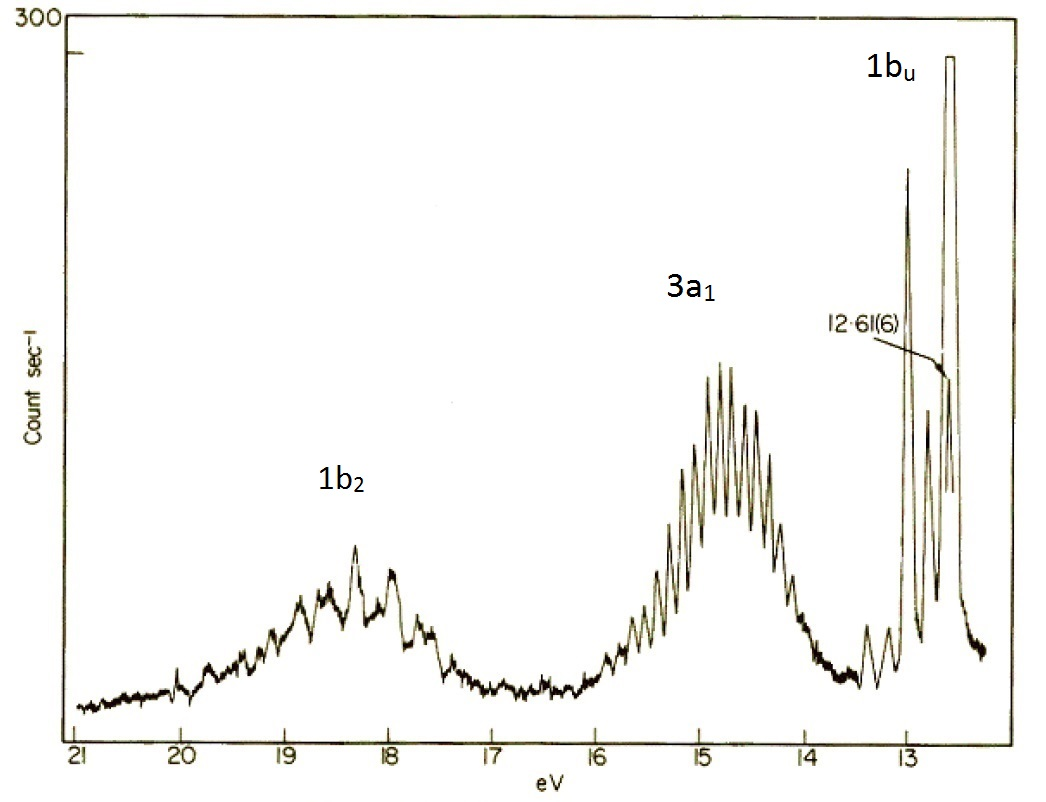
\includegraphics[width=2in]{img/PES_of_H2O.jpg}
\end{center}
\captionof{figure}{Photoionization spectrum of water in the gas phase (in eV). Source: Wikimedia Commons.}
\label{fig:water_pes}
}
The importance of Koopmans' theorem is that it build a bridge to experiments that measure the IP and EA of molecules.
For example, photoelectron spectroscopy, can measure the ionization potential (also called the binding energy) of electrons in different orbitals.
In this spectroscopy, a molecule is ionized with a high energy photon and one electron is released with kinetic energy equal to the energy of the photons ($h \nu$) minus the binding energy, $h \nu - IP$.
Therefore, it allows to measure the binding energy of different orbitals.
An example of the photoelectron spectrum of water in the gas phase is given in Fig.~\ref{fig:water_pes}.

The example below shows the Hartree--Fock orbital energies of the occupied and unoccupied orbitals of an isolated water molecule in the gas phase.
\begin{small}
\begin{verbatim}
  Water/Hartree-Fock
  Orbital Energies [Eh]
    ---------------------
    Doubly Occupied:                                                      

       1A1   -20.550918     2A1    -1.335304     1B2    -0.697799  
       3A1    -0.566090     1B1    -0.492954  

    Virtual:                                                              

       4A1     0.185103     2B2     0.255850     3B2     0.787301  
       5A1     0.851798     6A1     1.163709     2B1     1.200353  
       4B2     1.253480     7A1     1.444918     1A2     1.475588  
       3B1     1.674083     8A1     1.867861     5B2     1.931955  
       6B2     2.446380     9A1     2.483524     4B1     3.283306  
       2A2     3.336170    10A1     3.506961    11A1     3.862825  
       7B2     4.144454  

    Final Occupation by Irrep:
             A1    A2    B1    B2 
    DOCC [     3,    0,    1,    1 ]

  @RHF Final Energy:   -76.02665366185380

   => Energetics <=

    Nuclear Repulsion Energy =              9.1681932964243487
    One-Electron Energy =                -123.1035625229022514
    Two-Electron Energy =                  37.9087155646241101
    Total Energy =                        -76.0266536618537998
\end{verbatim}
\end{small}

The lowest ionization potential of water is estimated according to Koopmans' theorem from the energy of the highest occupied MO (HOMO, labeled 1b$_1$), which has an energy of $-0.493$ \Eh.
The corresponding IP is equal to 0.493 \Eh = 13.4 eV, a value that compares well with the experimental gas-phase IP (ca. 12.6 eV, indicated in the figure).
The ionization potential for the second orbital (labeled 3a$_1$) is 0.566 \Eh = 15.4 eV.
This corresponds to the  middle broad band in the spectrum centered around 15 eV.
Note that Koopmans' theorem applied to the Hartree--Fock solution also predicts that the anion \ce{H2O-} is unstable with respect to the process ionization process
\begin{center}
\ce{H2O- -> H2O + e-} 
\end{center}
since the energy of the first unoccupied orbital (virtual) is positive (0.185 \Eh).


%\section*{Summary}
%\begin{ibox}
%\begin{myitems}
%\item The wave function of .
%\item The \textbf{Hamiltonian operator} [$\hat{H}$]. Operators are mathematical objects that perform operations of function. Given an operator $\hat{O}$, when we apply it to a function $f(x)$ it returns another function $g(x)$, $\hat{O}f(x) = g(x)$.
%\item The \textbf{imaginary unit} [$i$]. 
%\item The \textbf{reduced Planck constan} [$\hbar = h / 2\pi$, pronounced ``h-bar''].
%\end{myitems}
%\end{ibox}



%Practical considerations
%Hartree-Fock self-consistent-field (HF SCF) usually converges fairly well with a good initial guess
%Stretched bonds, diradicals, transition metals, high-spin states, etc., can cause problems for convergence
%In high-symmetry cases, the program can guess the wrong orbital occupations, and then have trouble recovering from this to get the desired solution
%Not guaranteed to land on a local minimum in C space; can check by running a Hartree-Fock stability analysis (useful but not commonly done). However, even this doesn’t guarantee you’re not in some other local minimum (esp. for high-symmetry cases)
%User is responsible for making sure the orbital occupations are reasonable and the spin state is correct. Many students don’t know that the ground state of O2 is a triplet, not a singlet. The programs don’t know about this!
%     
%Improving Convergence
%Most codes use “direct inversion of the iterative subspace” (DIIS) to improve convergence (improves guess for the next step)
%The quality of the guess density makes a big difference. Core Hamiltonian (no initial density) is quite poor. Hückel and GWH ok; superposition of atomic densities (SAD) seems best when available
%Using MO's from one geometry as guesses for a nearby geometry (or neutral orbitals as a guess for a cation or anion, or singlet orbitals as a guess for a triplet) works well

\end{document}